% !TeX root = ../main.tex

\section{Homework \#5 [2025-10-09]}

\begin{problem}
  Verify the key step for proving the GML theorem:
  \[
    \ab(\sum_{j=1}^n \pdv*{}{t_j}) \longrightarrow n\pdv*{}{t_n}
  \]
  explicitly. Consider $n = 2$, and do the following
  \begin{enumext}
    \item Carry out the integration-by-path for each $t_j$.
    \item Show that for all $j$'s the final results are the same, i.e.,
    independent on $j$.
  \end{enumext}
\end{problem}
\begin{solution}\leavevmode
  \begin{enumext}
    \item Denote
    \[
      F(t_1, t_2)
    = \braket<0|\mathcal T[\phi_\text I(t_1) \phi_\text I(t_2) U]|0>, \quad
    \]
    where $U$ is the interaction picture evolution operator and $\mathcal T$ is
    the time-ordering operator. To simplify, define the unordered pieces
    \[
      A(t_1, t_2) = \braket<0|\phi_\text I(t_1) \phi_\text I(t_2) U|0>, \qq{and}
      B(t_1, t_2) = \braket<0|\phi_\text I(t_2) \phi_\text I(t_1) U|0>.
    \]
    Then, by definition of $\mathcal T$, we have
    \[
      F(t_1, t_2) = \theta(t_1 - t_2) A(t_1, t_2) +
                    \theta(t_2 - t_1) B(t_1, t_2),
    \]
    where $\theta$ is the Heaviside function.
    Now act $(\pdif{t_1} + \pdif{t_1})$ on $F$
    \begin{align*}
      \pdv F{t_1} + \pdv F{t_2} &
    = \theta(t_1 - t_2) \ab(\pdv A{t_1} + \pdv A{t_2}) +
      \theta(t_2 - t_1) \ab(\pdv B{t_1} + \pdv B{t_2}) +
      \delta(t_1 - t_2) (A - B)\\ &
    = \theta(t_1 - t_2) \ab(\pdif{t_1} A + \pdif{t_2} A) +
      \theta(t_2 - t_1) \ab(\pdif{t_1} B + \pdif{t_2} B),
    \end{align*}
    where the last term vanishes since $(A - B)|_{t_1=t_2} = 0$.
    Then, consider the integration
    \par \noindent
    \begin{minipage}{.72\linewidth}
    \begin{align*}
      I & = \int_{-\infty}^0 \d t_1 \int_{-\infty}^0 \d t_2
            (\pdif{t_1} + \pdif{t_2}) F(t_1, t_2)\\
        & = \underbrace{\int_{-\infty}^0 \d t_2 \int_{t_2}^0 \d t_1
            (\pdif{t_1} A + \pdif{t_2} A)}_\text{Region 1: $t_1 > t_2$}
          + \underbrace{\int_{-\infty}^0 \d t_1 \int_{t_2}^0 \d t_2
            (\pdif{t_1} B + \pdif{t_2} B)}_\text{Region 2: $t_2 > t_1$}.
    \end{align*}
    \end{minipage}
    \begin{minipage}{.24\linewidth} \centering
    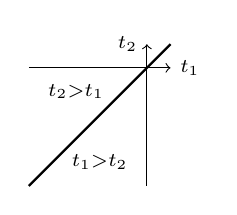
\begin{tikzpicture}[scale = .6]
      \draw [->] (-2.5,0) -- (.5,0) node [right] {$\scriptstyle t_1$};
      \draw [->] (0,-2.5) -- (0,.5) node [left] {$\scriptstyle t_2$};
      \draw [thick] (.5,.5) -- (-2.5,-2.5);
      \node at (-1.5,-.5) {$\scriptstyle t_2 > t_1$};
      \node at (-1,-2) {$\scriptstyle t_1 > t_2$};
    \end{tikzpicture}
    \end{minipage}
    \par\noindent
    Consider Region I
    \begin{align*}
      I_1 & = \int_{-\infty}^0 \d t_2 \int_{t_2}^0 \d t_1 \pdif{t_1} A(t_1, t_2)
            + \int_{-\infty}^0 \d t_2 \int_{t_2}^0 \d t_1 \pdif{t_2} A(t_1, t_2)\\
          & \xlongequal{\text{Leibniz integral rule}}
            \int_{-\infty}^0 \d t_2 [A(0, t_2) - A(t_2, t_2)] +
            \int_{-\infty}^0 \d t_2 \ab[A(t_2, t_2) -
              \odv*[fun]{\int_0^{t_2} A(t_1, t_2) \d t_1}{t_2}]\\
          & = \int_{-\infty}^0 \d t_2 A(0, t_2) - \ab[
              \int_0^0 A(t_1, 0) \d t_1 -
              \int_0^{-\infty} A(t_1, -\infty) \d t_1]
            = \int_{-\infty}^0 \d t_2 A(0, t_2).
    \end{align*}
    The last term vanishes due to the boundary condition.
    Similarly, for Region II, the integration can be written as
    \[
      I = \int_{-\infty}^0 \d t_2 A(0, t_2) + \int_{-\infty}^0 \d t_1 B(0, t_1)
        = \int_{-\infty}^0 \d t_2 A(0, t_2) + \int_{-\infty}^0 \d t_1 A(t_1, 0)
        = 2\int_{-\infty}^0 \d t_1 A(0, t_1).
    \]
    In the last step, both the integral region and the variables are switched.
    Since
    \[
      F(t_1, 0) = \theta(t_1 - 0) A(t_1, 0) + \theta(0 - t_1) B(t_1, 0)
    = A(0,t_1),
    \]
    integral over $t_2$ to $\pdif{t_2} F(t_1, t_2)$
    \[
      \int_{-\infty}^0 \d t_2 \pdif{t_2} F(t_1, t_2)
    = F(t_1, 0) - F(t_1, -\infty) = F(t_1, 0) = A(0,t_1).
    \]
    So, we have
    \[
      I = 2\int_{-\infty}^0 \d t_1 \int_{-\infty}^0 \d t_2
            \pdif{t_2} F(t_1, t_2)
        = \int_{-\infty}^0 \d t_1 \int_{-\infty}^0 \d t_2
            (\pdif{t_1} + \pdif{t_2}) F(t_1, t_2).
    \]
    Then we obtain
    \[
      \pdif{t_1} + \pdif{t_2} = 2\pdif{t_2}, \qq{i.e.,}
      \ab(\sum_{j=1}^2 \pdif{t_j}) \longrightarrow 2 \pdif{t_2}.
    \]
    \item Denote $T = \frac12(t_1 + t_2)$, $\tau = t_1 - t_2$.
    Holding $\tau$ fixed,
    \[
      \pdif{t_1}\big|_\tau = \pdv*{}T \pdv T{t_1} = \frac12\pdv*{}T, \qq{and}
      \pdif{t_2}\big|_\tau = \pdv*{}T \pdv T{t_2} = \frac12\pdv*{}T
    \]
    So, we have $2\pdv*{}{t_1}|_\tau = 2\pdv*{}{t_2}|_\tau = \pdif T$,
    hence the result is independent of which $t_j$ is chosen.
  \end{enumext}
\end{solution}

\begin{problem}[The two-spin problem]
  Consider two spin-$1/2$'s, $\hat s_a = \hat s_b = \frac12$,
  which are coupled to each other via an exchange interaction $J$
  and are presumed to be acted upon by a homogeneous magnetic field.
  We describe them in terms of the correspondingly simplified Heisenberg model
  \[
    \mathcal H_0  = \ab(\frac{J_\bot}{2}(\hat s_a^{++}\hat s_b^-
                  + \hat s_a^-\hat s_b^{++}) + J_z\hat s_z^z\hat s_b^z)
                  - h_z(\hat s_a^z + \hat s_b^z).
  \]
  The parameter choice is to ensure that when $J_\bot = J_z$
  the first term reduces to the Heisenberg interaction.
  For this problem, we take $J_\bot = 0$, which is called the Ising limit,
  $b = 0$ and also assume $J_z > 0$
  (for this problem, the sign does not make much difference,
  but it will be important when we turn on $J_\bot$).
  Next, consider a transverse field as the perturbation
  \[
    \delta \mathcal H = -h_x(\hat s_a^x + \hat s_b^x).
  \]
  Consider the two-spin COBS, $U_{g2} = \{\hat I, \hat S^\alpha, \hat\eta, \hat B_S^\alpha, \hat B_A^\alpha, \hat D^\alpha\}$ defined as
  \[\begin{array}{l@{~}c@{~}l}
    \hat S_{ab}^\alpha    & = & \hat s_a^\alpha + \hat s_b^\alpha,~
    \hat\eta_{ab}^\alpha    = \hat s_a^\alpha - \hat s_b^\alpha,\\
    \hat B_{A,ab}^\gamma  & = & 2\epsilon_{\alpha\beta\gamma}
                              \hat s_a^\alpha \hat s_b^\beta,\\
    \hat B_{S,ab}^\gamma  & = & 2\epsilon_{\alpha\beta\gamma}^2
                              \hat s_a^\alpha \hat s_b^\beta,\\
    \hat D_{ab}^\alpha    & = & 2\hat s_a^\alpha \hat s_b^\alpha,
  \end{array}\]
  where the Einstein summation notation over dummy indices is assumed.
  \begin{enumext}
    \item Determine the exact ground state(s) of $\mathcal H_0$,
    specify the degeneracy, if any, by diagonalization, i.e.,
    rewrite $\mathcal H_0$ as a $4 \times 4$ matrix.
    \item Parameterize the degenerate ground state subspace;
    compute expectation values of COBS elements for a parameterized state;
    try to use symmetry as a guide,
    only $5$ out of the $15$ operators have none-zero values;
    for two-body operators, use the cumulant expression.
    \item Determine the exact ground state energy
    and the ground state wavefunction for
    $\mathcal H = \mathcal H_0 + \delta \mathcal H$, assuming $J_z > 4h_x > 0$;
    also compute expectation values for the COBS elements;
    carry out the Taylor expansion for $\braket<\hat S^x>$
    to the first order, to determine the transverse field susceptibility
    $\chi_x = \pdv{\braket<\hat S^x>}{h_x}\Big|_{h_x\to0}$;
    determine the ground state in the same limit $\ket|\Psi>\big|_{h_x\to0^+}$.
    \item Try to use the perturbative VES Eq. \eqref{5.6.10}
    \begin{equation}
      0 = \braket<[\delta\mathcal H, \hat u^{\alpha_0}]>_0
        + \sum_\alpha \delta\braket<\hat u^\alpha>
          \braket<\{\hat u^\alpha, [\mathcal H, \hat u^{\alpha_0}]\}>_0
        + \sum_{\gamma\beta} \braket<\delta\hat u^\gamma>
          \braket<\delta\hat u^\beta>
          \braket<\{\hat u^\gamma,
            [\mathcal H, \{\hat u^{\alpha_0}, \hat u^\beta\}]\}>_0 + \ldots,
      \tag{5.6.10} \label{5.6.10}
    \end{equation}
    to do the computation, starting from a parameterized state,
    and express the transverse field susceptibility $\chi_x$
    as a function of COBS expectation values;
    determine the parameterized state with the largest $\chi_x$ and
    compare with the diagonalization results you obtained in the previous question.
    \item You should find that the fully entangled triplet state has the largest
    $\chi_x$, try to discuss the reason based on your calculation results.
  \end{enumext}
\end{problem}
\begin{solution}
  Since we take $J_\bot = 0$, and omit the perturbation term. The Hamiltonian
  becomes
  \[
    \mathcal H_0 = J_z \hat s_a^z \hat s_b^z.
  \]
  \begin{enumext}
    \item Recall $\hat s^z = \frac12\sigma^z$, then
    $\hat s_a^z\hat s_b^z = \frac14\sigma_a^z\sigma_b^z$.
    Taking the basis
    \[
      \{\ket|\uparrow\uparrow>,\    \ket|\uparrow\downarrow>,\
        \ket|\downarrow\uparrow>,\  \ket|\downarrow\downarrow>\}.
    \]
    Therefore, the eigenenergies, i.e., the diagonal matrix elements, are
    \[
      E(\uparrow\uparrow)     = \frac{J_z}{4}, \quad
      E(\uparrow\downarrow)   = -\frac{J_z}{4}, \quad
      E(\downarrow\uparrow)   = -\frac{J_z}{4}, \quad
      E(\downarrow\downarrow) = \frac{J_z}{4}.
    \]
    So, $\mathcal H_0$ can be written into a $4\times4$ diagonal matrix
    \[
      \mathcal H_0
    = \pdiagmat[empty = {}]
        {\frac{J_z}{4}, -\frac{J_z}{4}, -\frac{J_z}{4}, \frac{J_z}{4}}.
    \]
    The ground states are
    $\ket|\uparrow\downarrow>$ and $\ket|\downarrow\uparrow>$.
    Since the two lowest eigenvalues are equal, the degeneracy is $2$.
    \item Parameterize a normalized general state in the ground subspace as
    \[
      \ket|\psi(\theta, \phi)> = \cos\frac\theta2 \ket|\uparrow\downarrow>
                + \upe^{\iu\phi} \sin\frac\theta2 \ket|\downarrow\uparrow>.
    \]
    The general is normalized.
    The non-zero values of the 5 COBS elements are listed as follows
    \[\begin{array}{l@{~}c@{~}l<{,}@{\quad}l@{~}c@{~}l}
      \hat \eta^z & = & \hat s_a^z - \hat s_b^z &
      \braket<\hat\eta^z>
    = |\cos(\theta/2)|^2 - |\upe^{\iu\theta}\sin(\theta/2)|^2
    = \cos\theta,\\
      \hat D^x & = & 2\hat s_a^x\hat s_b^x      &
      \braket<\hat D^x>
    = \Re\{[\cos(\theta/2)]^*\upe^{\iu\theta}\sin(\theta/2)\}
    = \frac12\sin\theta\cos\phi,\\
      \hat D^y & = & 2\hat s_a^y \hat s_b^y     &
      \braket<\hat D^y> = \braket<\hat D^x> = \frac12\sin\theta\cos\phi,\\
      \hat D^z & = & 2\hat s_a^z \hat s_b^z     &
      \braket<\hat D^z> = -\frac12,\\
      \hat B_A^z & = & 2(\hat s_a^x\hat s_b^y - \hat s_a^y\hat s_b^x) &
      \braket<\hat B_A^z>
    = -2\Im\{[\cos(\theta/2)]^*\upe^{\iu\theta}\sin(\theta/2)\}
    = -\sin\theta\sin\phi.
    \end{array}\]
    \item The total Hamiltonian is
    \def \0 {\frac{J_z}{4}}
    \def \1 {-\frac{h_x}{2}}
    \begin{align*}
      \mathcal H & = \mathcal H_0 + \delta \mathcal H
    = J_z \hat s_a^z \hat s_b^z - h_x (\hat s_a^x + \hat s_b^x)
    = J_z \hat s_a^z \hat s_b^z - h_x \hat S_x\\ & =
    \begin{pmatrix}
      \0 & \1 & \1 & 0  \\
      \1 & -\0 & 0 & \1 \\
      \1 & 0 & -\0 & \1 \\
      0 & \1 & \1 & \0
    \end{pmatrix} \sim
    \pdiagmat[empty = {}]
      {-\frac14\sqrt{J_z^2 + 16h_x^2}, -\frac{J_z}{4}, +\frac{J_z}{4},
       +\frac14\sqrt{J_z^2 + 16h_x^2}}.
    \end{align*}
    Therefore, the exact ground state energy is
    $E_0 = -\frac14\sqrt{J_z^2 + 16h_x^2}$.
    The exact ground eigenvector (wavefunction) can be expressed as
    \[
      \ket|\Psi_0> = \ket|\uparrow\uparrow> +
      \ab(\frac{J_z}{4h_x} - \frac{\sqrt{J_z^2 + 16h_x^2}}{4h_x})
      \ab(\ket|\uparrow\downarrow> + \ket|\downarrow\uparrow>) +
      \ket|\downarrow\downarrow>.
    \]
    The expectation values are
    \[\begin{array}{l@{~}c@{~}l<{,}@{\quad}
                    l@{~}c@{~}l<{,}@{\quad}
                    l@{~}c@{~}l}
      \braket<\hat S_x> & = & \frac{h_x}{\sqrt{(J_z/4)^2 + h_x^2}} &
      \braket<\hat S^y> & = & \braket<\hat S^z> = 0 &
      \braket<\hat \eta>& = & 0,\\
      \braket<\hat B_A^\alpha> & = & \braket<\hat B_s^\alpha> = 0 &
      \braket<\hat D^x> & = & \braket<\hat D^y> = \frac12 &
      \braket<\hat D^z> & = & \frac{2\lambda^2 - 1}{2(1 + 2\lambda^2)},
    \end{array}
    \]
    where $\lambda = \frac{\sqrt{(J_z/4)^2 + h_x^2} - J_z/4}{\sqrt2h_x}$.
    Under the limitation of $h_x \to 0$, the ground energy can be expanded as
    \[
      E_1 \approxeq -\frac{J_z}{4} - \frac{2h_x^2}{J_z} + \mathcal O(h_x^4),
    \]
    and the expectation of $\braket<\hat S^x>$ under this limitation becomes
    \[
      \lim_{h_x\to0} \braket<\hat S^x> = \frac{4h_x}{J_z},
    \]
    and the transverse field susceptibility $\chi_x = 4/J_z$, the ground state
    \[
      \lim_{h_x\to0} \ket|\Psi> = \frac1{\sqrt2} \ket|\uparrow\uparrow> +
                                  \frac1{\sqrt2} \ket|\downarrow\downarrow>,
    \]
    where the normalization factor is $\frac1{\sqrt2}$.
    \item We only consider the top 2 orders of the VES equation.
    Choose $\hat u^{\alpha_0} = \hat S^x$,then
    \[
      \braket<[\delta \mathcal H, \hat S^x]>_0
    = -h_x \braket<[\hat S^x, \hat S^x]>_0 = 0,
    \]
    and the VES equation becomes
    \[
      \sum_\alpha \delta\braket<\hat u^\alpha>
      \braket<\{\hat u^\alpha, [\mathcal H_0, \hat u^{\alpha_0}]\}>_0 = 0.
    \]
    \begin{enumext}
      \item Compute $[\mathcal H_0, \hat S^x]$.
      \[
        [\mathcal H_0, \hat S^x]
      = J_z [\hat S_a^z \hat S_b^z, \hat S_a^x + \hat S_b^x]
      \xlongequal[{[\hat S_b^z, \hat S_b^x] = i\hat S_b^y}]
        {[\hat S_a^z, \hat S_a^x] = i\hat S_a^y}
        \iu J_z (\hat S_a^y \hat S_b^z + \hat S_a^z \hat S_b^y).
      \]
      \item Choose the relevant Ooerator $\hat u^\alpha = \hat B_A^y$.\\
      From symmetry analysis, the operator is expressed as
      $\hat B_A^y = 2(\hat S_a^z \hat S_b^x - \hat S_a^x \hat S_b^z)$.
      Then
      \[
        \braket<\{\hat B_A^y, [\mathcal H_0, \hat S^x]\}>_0
      = -\iu J_z \braket<\hat D^x>_0, \qq{and}
        \delta\braket<\hat B_A^y> = -2\delta\braket<\hat S^x>,
      \]
      where $\hat D^x = 2\hat S_a^x \hat S_b^x$.
    \end{enumext}
    Substitute them into the VES equation
    \[
      0 = 0 + \delta\braket<\hat B_A^y> \cdot (-\iu J_z \braket<\hat D^x>_0)
        = (-2\delta\braket<\hat S^x>)(-iJ_z \braket<\hat D^x>_0),\quad
          \braket<\hat S^x> \approxeq \delta \braket<\hat S^x>
        = \frac{2h_x}{J_z}(1 + 2\braket<\hat D^x>_0).
    \]
    Then, the transverse susceptibility
    \[
      \chi_x = \pdv{\hat S^x}{h_x} = \frac2{J_z}(1 + 2\braket<\hat D^x>_0)
    = \frac2{J_z} \ab(1 + 2\times\frac12) = \frac4{J_z},
    \]
    which is the same as the previous question.
    \item The triplet state $\ket|1,0>$ maximizes $\chi_x$ because it achieves
    the largest $\braket<\hat D^x>_0 = 1/2$ in the susceptibility formula
    $\chi_x = (2/J_z)(1 + 2\braket<\hat D^x>_0)$, yielding $\chi_x = 4/J_z$.
    Its symmetric structure provides optimal matrix elements for transverse
    field coupling.
  \end{enumext}
\end{solution}

\begin{problem}[extra credit, I don't see the answer right way yet
                but I think both approaches should agree]
  Use the results of section 5.7.1.5 to compute the propagator of a driven harmonic
  oscillator discussed in section 5.8.1.1. You may change the creation /
  annihilation operator representation into the $x$/$p$ representation if
  needed; i.e., consider the following Hamiltonian and perturbation,
  \[
    \hat H_0 = \omega\ab(b^\dagger b + \frac12), \quad
    \hat V(t) = \bar z(t)b(t) + b^\dagger(t) z(t),
  \]
  and prove that the propagator is
  \[
    S[\bar z, z] = \braket*\bigg<0|\mathcal T\exp\ab(-\iu\int_{-\infty}^\infty
      \d t[\bar z(t) b(t) + b^\dagger(t) z(t)])|0>
  = \exp\ab[\iu\int_{-\infty}^\infty \d t \d t' \bar z(t) G(t - t') z(t')],
  \]
  where $G(t - t') = -\iu\theta(t - t') \upe^{-\iu\omega(t-t')}$.
  \begin{remark}
    Seems all contributions directly step from the factor
    $\exp\{\frac\iu\hbar S[x_c l(t), \dot x(t), t]\}$.
    Connect the contribution to the $G(t - t')$ in the absence of the external
    drive $z(t)$.
  \end{remark}
\end{problem}
\begin{solution}
  The time evolution of the creation and annihilation operators in Dirac
  picture can be written as
  \[
    b_\text I(t) = b\upe^{-\iu\omega t}, \qq{and}
    b_I^\dagger(t) = b^\dagger \upe^{\iu\omega t}.
  \]
  The propagator can be written as a vacuum-to-vacuum amplitude in the Dirac picture
  \[
    S[\bar z, z]
  = \braket*<0|\mathcal T\exp\ab(-\iu\int_{-\infty}^\infty \hat V_\text I(t) \d t)|0>,
  \]
  where $\hat V_\text I(t)$ is the Dirac picture perturbation
  \[
    \hat V_\text I(T) = \upe^{\iu\hat H_0t} \hat V(t) \upe^{-\iu\hat H_0t}
  = \bar z(t) b\upe^{-\iu\omega t} + b^\dagger z(t) \upe^{\iu\omega t}
  \]
  the above expression used the following identities
  \[
    \upe^{\iu\hat H_0 t} b \upe^{-\iu\hat H_0 t}
  \xlongequal[{[\iu\hat H_0t,b] = -\iu\omega tb}]{\text{BCH identity}}
    b\upe^{-\iu\omega t}, \qq{and}
    \upe^{\iu H_0 t} b^\dagger \upe^{-\iu\hat H_0t}
  \xlongequal[{[\iu\hat H_0t,b^\dagger] = \iu\omega tb^\dagger}]
    {\text{BCH identity}} b^\dagger \upe^{\iu\omega t}.
  \]
  Then, we compute the vacuum expectation
  \begin{align*}
    \braket<0|\mathcal T[\hat V_\text I(t_1) \hat V_\text I(t_2)]|0> &
  = \theta(t_1 - t_2) \upe^{-\iu\omega(t_1-t_2)} \bar z(t_1) z(t_2)
  + \theta(t_2 - t_1) \upe^{-\iu\omega(t_2-t_1)} \bar z(t_2) z(t_1)\\ &
  = 2\theta(t_1 - t_2) \upe^{-\iu\omega(t_1-t_2)} \bar z(t_1) z(t_2).
  \end{align*}
  The $\mathcal S$-matrix can be expanded as
  \[
    \mathcal S
  = \mathcal T\exp\ab(-\iu\int_{-\infty}^\infty \hat V_\text I(t) \d t)
  = 1 + (-\iu) \int \d t_1 \hat V_\text I(t_1)
      + \frac{(-\iu)^2}{2} \int \d t_1 \int \d t_2
        \mathcal T [\hat V_\text I(t_1)\hat V_\text I(t_2)] + \cdots.
  \]
  Then, the connected part of the vacuum expectation is
  \[
    \log\braket<0|\mathcal S|0> = -\frac12 \int \d t_1 \d t_2
    \braket<0|\mathcal T[\hat V_\text I(t_1) \hat V_\text I(t_2)]|0> + \cdots
  = -\int \d t_1 \d t_2 \theta(t_1 - t_2)
    \upe^{-\iu\omega(t_1-t_2)} \bar z(t_1) z(t_2),
  \]
  where only the contractions between $b$ and $b^\dagger$ are non-zero.
  Therefore
  \[
    \braket<0|\mathcal S|0> = \exp\ab(-\int \d t \d t' \theta(t - t')
      \upe^{-\iu\omega(t - t')} \bar z(t) z(t')).
  \]
  We define the retarded Green function
  \[
    G(t - t') = -\iu\theta(t - t') \upe^{-\iu\omega(t-t')}.
  \]
  Then, the propagator can be expressed as
  \[
    \mathcal S[\bar z, z]
  = \exp\ab[\iu\int_{-\infty}^\infty \d t \d t' \bar z(t) G(t - t') z(t')],
  \]
  where $G(t - t') = -\iu\theta(t - t') \upe^{-\iu\omega(t-t')}$.
\end{solution}